\documentclass[11pt,oneside]{article}

	% History ================================================================
	% 2023.06.03 - Modified from Chase Murray's version
	% ========================================================================

    % STANDARD PACKAGES ======================================================
    \usepackage{datetime}
    \usepackage{graphicx}
    % \usepackage{ctex} % Allow Chinese characters
    \usepackage[utf8]{inputenc}
    \usepackage[american]{babel}
    \usepackage{amssymb}
    \usepackage[intlimits]{amsmath}
    \usepackage{amsfonts}
    \usepackage{amsthm}
    \usepackage{array}
    \usepackage{mdwlist}        
    \usepackage[labelsep=quad,indention=10pt]{subfig}
    \usepackage{algorithm}
    \usepackage[noend]{algpseudocode}
    \usepackage{lscape}
    \usepackage{rotating} % Allows \begin{sideways} \end{sideways} for vertical table headers.    
    \usepackage{threeparttable} % Allow footnotes in tables.    
    \usepackage{tabularx}
    \usepackage{multirow} % Allow table cells to span multiple rows/cols.
    \usepackage{makecell}
    \usepackage{longtable}
    \usepackage{url} % Allow \url{} and \href{url}{name}
    \usepackage{verbatim}    
    \usepackage{enumerate} % http://www.tex.ac.uk/cgi-bin/texfaq2html?label=enumerate
    \usepackage{color} % Allow colored fonts
    \usepackage[toc,page]{appendix}

    \usepackage{bm}

    \usepackage{tikz}
    \usepackage{diagbox}
    \usepackage{lastpage} % \pageref{LastPage} = total number of pages.
    \usepackage{ifthen}        
    \usepackage{setspace} % Allows \singlespacing, \onehalfspacing, \doublespacing 
    \usepackage{listings} % Allows formatting of Python code (and other languages)
    \usepackage{wrapfig}
    \usepackage[normalem]{ulem} % Allows strikethrough (\sout{text to strike})
    % \usepackage{subfigure}        % Allows subfigs/subfloats


    \usepackage{xcolor,colortbl}    % http://ctan.org/pkg/xcolor
    % \usepackage[table]{xcolor}    % https://tex.stackexchange.com/questions/50349/color-only-a-cell-of-a-table
    
    % Make sure that {color} and {xcolor} are called before mdframed
    \usepackage[framemethod=TikZ]{mdframed}    % Allows colored textbox

    \usepackage{lipsum}                     % Dummy text
    % ========================================================================

    % DEFINE PROGRAMMING FORMAT ++++++++++++++++++++++++++++++++++++++++++++++
        \lstset{language=Python}          % Set your language (you can change the language for each code-block optionally)

        \definecolor{mygreen}{rgb}{0,0.6,0}
        \definecolor{mygray}{rgb}{0.5,0.5,0.5}
        \definecolor{mymauve}{rgb}{0.58,0,0.82}

        \lstset{
          backgroundcolor=\color{gray!05!white},   % choose the background color; you must add \usepackage{color} or \usepackage{xcolor}; should come as last argument
          basicstyle=\ttfamily,                    % the size of the fonts that are used for the code
          breakatwhitespace=false,                 % sets if automatic breaks should only happen at whitespace
          breaklines=true,                         % sets automatic line breaking
          captionpos=t,                            % sets the caption-position to bottom
          commentstyle=\color{black},              % comment style
          deletekeywords={...},                    % if you want to delete keywords from the given language
          escapeinside={\%*}{*)},                  % if you want to add LaTeX within your code
          extendedchars=true,                      % lets you use non-ASCII characters; for 8-bits encodings only, does not work with UTF-8
          frame=single,                               % adds a frame around the code
          keepspaces=true,                         % keeps spaces in text, useful for keeping indentation of code (possibly needs columns=flexible)
          % keywordstyle=\color{blue},             % keyword style
          language=Python,                         % the language of the code
          morekeywords={*,...},                    % if you want to add more keywords to the set
          numbers=left,                            % where to put the line-numbers; possible values are (none, left, right)
          numbersep=5pt,                           % how far the line-numbers are from the code
          % numberstyle=\tiny\color{mygray},       % the style that is used for the line-numbers
          rulecolor=\color{black},                 % if not set, the frame-color may be changed on line-breaks within not-black text (e.g. comments (green here))
          showspaces=false,                        % show spaces everywhere adding particular underscores; it overrides 'showstringspaces'
          showstringspaces=false,                  % underline spaces within strings only
          showtabs=false,                          % show tabs within strings adding particular underscores
          stepnumber=1,                            % the step between two line-numbers. If it's 1, each line will be numbered
          % stringstyle=\color{mymauve},           % string literal style
          tabsize=4,                               % sets default tabsize to 2 spaces
          % title=\lstname,                        % show the filename of files included with \lstinputlisting; also try caption instead of title
          xleftmargin=35pt,
          xrightmargin=15pt, 
          aboveskip=0pt,
          belowskip=5pt
        }
    % ++++++++++++++++++++++++++++++++++++++++++++++++++++++++++++++++++++++++

    % DEFINE/RENEW SOME ENVIRONMENTS =========================================    
        \renewenvironment{abstract}
          {\normalfont\footnotesize
            \list{}{\labelwidth0pt
              \leftmargin20pt \rightmargin\leftmargin
              \listparindent\parindent \itemindent0pt
              \parsep0pt
              \let\fullwidthdisplay\relax
            }
            \item[\hskip\labelsep\bfseries\abstractname:] %
        }{
          \endlist}

        \newcommand{\keywordsname}{Keywords}
        \newenvironment{keywords}
          {\normalfont\footnotesize
            \list{}{\labelwidth0pt
              \leftmargin20pt \rightmargin\leftmargin
              \listparindent\parindent \itemindent0pt
              \parsep0pt
              \let\fullwidthdisplay\relax}
            \item[\hskip\labelsep\bfseries\keywordsname:]}{\endlist}

        \newcommand{\dochistname}{History}
        \newenvironment{DocHistory}
          {\normalfont\footnotesize
            \list{}{\labelwidth0pt
              \leftmargin20pt \rightmargin\leftmargin
              \listparindent\parindent \itemindent0pt
              \parsep0pt
              \let\fullwidthdisplay\relax}
            \item[\hskip\labelsep\bfseries\dochistname:]}{\endlist}
    % ========================================================================    

    % DEFINE PAGE FORMATTING +++++++++++++++++++++++++++++++++++++++++++++++++
        % Select Line Spacing:
        \singlespacing
        % \onehalfspacing        
        % \doublespacing    

        % Margins:
        \usepackage[letterpaper,left=1.0in,top=1.0in,right=1.0in,bottom=1.0in]{geometry}
    
        % Page Style
        \pagestyle{plain}    % Includes page number
        %\pagestyle{empty}    % Completely blank                

        % By default all math is set to inline mode. The \displaystyle command
        % ensures that we don't get small fractions or summations with limits
        % on the sides.
        \everymath{\displaystyle}    
        
        % http://tex.stackexchange.com/questions/5223/command-for-argmin-or-argmax
        \DeclareMathOperator*{\argmin}{arg\,min}

        % Allow flalign items to be split over multiple pages:
        \allowdisplaybreaks[1]   % See ftp://ftp.ams.org/pub/tex/doc/amsmath/amsldoc.pdf    
    % ++++++++++++++++++++++++++++++++++++++++++++++++++++++++++++++++++++++++

    % DEFINITION, THEOREM, AND LEMMA +++++++++++++++++++++++++++++++++++++++++

        \theoremstyle{definition}
            \newtheorem{definition}{Definition}[section]
            \newtheorem*{example}{Example}
            \newtheorem{problem}{Problem}[section]
            \newtheorem*{solution}{Solution}
            \newtheorem{hypothesis}{Hypothesis}[section]
        \theoremstyle{plain}
            \newtheorem{theorem}{Theorem}[section]
            \newtheorem{corollary}{Corollary}[theorem]
            \newtheorem{lemma}[theorem]{Lemma}
            \newtheorem{conjecture}{Conjecture}
            \newtheorem{proposition}{Proposition}
        \theoremstyle{remark}
            \newtheorem*{remark}{Remark}

    % ++++++++++++++++++++++++++++++++++++++++++++++++++++++++++++++++++++++++

    % CUSTOM MACROS ++++++++++++++++++++++++++++++++++++++++++++++++++++++++++

        % This is how you may create a new variable:
        % \newcommand{\docjunk}{ text to display }
        
        % See https://gist.github.com/benkehoe/c46647134d4bbd514869
        % for more examples.

        % Create a box marked ``To Do'' around text.
        % \todo{  insert text here  }.
        \newcommand{\todo}[1]{\vspace{5 mm}\par \noindent
        \marginpar{\textsc{to do}}
        \framebox{\begin{minipage}[c]{0.95 \textwidth}
        \tt\begin{center} #1 \end{center}\end{minipage}}\vspace{5 mm}\par}

        % Create an empty box marked ``Result'' in the margin.
        % Specify the number of empty rows.
        % \result{8 em}.
        \newcommand{\result}[1]{\vspace{5 mm}\par \noindent
        \marginpar{\textsc{Result}} $\qquad\qquad$
        \framebox{\begin{minipage}[c]{0.75 \textwidth}
        \tt\begin{center} \vspace{#1} \end{center}\end{minipage}}\vspace{5 mm}\par}

        % Color selected text in red font.
        % \alert{text to color}
        \newcommand{\alert}[1]{{\color{red}#1}}

        % Color selected text in blue font.
        % \edited{text to color}
        \newcommand{\edited}[1]{{\color{blue}#1}}

        % Color selected text and add a "FIXME" note in the margin.
        % \fixme{text to color}
        \newcommand{\fixme}[1]{{\color{red}#1}
            \marginpar{\textsc{\color{red}fixme}}}

        % Color selected text (optional) and add a note in brackets.
        % \note[selected text]{comments}
        % \note{comments}
        \renewcommand{\note}[2][]{
            {\color{blue}#1 %
            [\textsc{note}:~#2]}
        }
        
        % Color selected text (optional) and add a note from someone.
        % \notefrom[selected text]{from}{comments}
        % \notefrom{from}{comments}
        \newcommand{\notefrom}[3][]{
            {\color{green!50!black}#1 %
            [\textsc{from #2}:~#3]}
        }
        
        % Color selected text (optional) and add a note to someone.
        % \noteto[selected text]{to}{comments}
        % \noteto{to}{comments}
        \newcommand{\noteto}[3][]{
            {\color{red}#1 %
            [\textsc{to #2}:~#3]}
        }

        % Color and Line Settings for Boxed Text
        \mdfsetup{
        % middlelinecolor=red,
        middlelinewidth=1pt,
        % linecolor=blue,
        % linewidth=1pt,
        backgroundcolor=orange!10!white,
        linecolor=orange!50!black,
        roundcorner=5pt}
        
        % Shortcut for referencing figures/tables:
        % Usage:  \figref{fig:name} --> Figure 1.
        \newcommand{\figref}[1]{\figurename~\ref{#1}}
        \newcommand{\tabref}[1]{\tablename~\ref{#1}}
    % ++++++++++++++++++++++++++++++++++++++++++++++++++++++++++++++++++++++++

    % SETUP TikZ +++++++++++++++++++++++++++++++++++++++++++++++++++++++++++++
        \usetikzlibrary{arrows,shapes,matrix}
        \usetikzlibrary{decorations.pathmorphing} 
        \usepgflibrary{plotmarks}
        \usetikzlibrary{patterns}  
        \usetikzlibrary{positioning} 
        \usetikzlibrary{snakes}  
        \tikzstyle{block}=[draw opacity=0.7,line width=1.4cm]
        
        % MORE STUFF TO ADD HERE?
    % ++++++++++++++++++++++++++++++++++++++++++++++++++++++++++++++++++++++++

    % SETUP BIBLIOGRAPHY +++++++++++++++++++++++++++++++++++++++++++++++++++++
    % [This section MUST be used if you have a bibliography.    ]
    % [Otherwise, leave this section commented out.        ]
    % \begin{comment}

        % FIXME -- EXPLAIN
        
        % Setup the Bibliography Style -- Select ONE of the following:
        % \usepackage{natbib}
        % \usepackage[sectionbib,square]{natbib}     %%% See natbib.pdf for explanation.
        % \usepackage[sectionbib,round]{natbib}
        \usepackage[square,numbers]{natbib}

        \bibliographystyle{plainnat}

        % Natbib setup for author-year style
        % \bibpunct has 1 optional and 6 mandatory arguments:
        %  [0.] The character preceding a post-note, default is a comma plus space. In redefining this character, 
        %     one must include a space if one is wanted. 
        %  1. the opening bracket symbol, default = (
        %  2. the closing bracket symbol, default = )
        %  3. the punctuation between multiple citations, default = ;
        %  4. the letter `n' for numerical style, or `s' for numerical superscript style, 
        %    any other letter for author-year, default = author-year;
        %  5. the punctuation that comes between the author names and the year
        %  6. the punctuation that comes between years or numbers when common author lists are suppressed (default = ,);

        % Natbib setup for author-year style
        \bibpunct[, ]{(}{)}{,}{a}{}{,}                % Use author names
        % \bibpunct[, ]{[}{]}{,}{n}{}{,}            % Use numbers
        
        \def\bibfont{\small}
        \def\bibsep{\smallskipamount}
        \def\bibhang{24pt}
        \def\newblock{\ }
        \def\BIBand{and}
    % \end{comment}
    % ++++++++++++++++++++++++++++++++++++++++++++++++++++++++++++++++++++++++

    % DOCUMENT INFO ++++++++++++++++++++++++++++++++++++++++++++++++++++++++++
        \newcommand{\docTitle}{}

        % List authors here, separated by \and 
        \newcommand{\docAuthor}{}
        % \newcommand{\docAuthor}{}

        \newcommand{\docAffil}{
            School of Management, Shanghai University, Shanghai, China
        }

        \newcommand{\docAbstract}{}

        \newcommand{\docKeyword}{}

        % This date will appear under the title.
        \newcommand{\docDate}{\today}       % {} --> don't show a date.
            
        % This date will appear in the page header:
        \newcommand{\draftDate}{\today}    % {\today} --> draft, {} --> finalized (hidden)
    
        % The image files should be saved here:
        \graphicspath{ {../../image/} }
    % ++++++++++++++++++++++++++++++++++++++++++++++++++++++++++++++++++++++++

    % DEFINE HEADER ++++++++++++++++++++++++++++++++++++++++++++++++++++++++++
        \usepackage{fancyhdr}
        \pagestyle{fancy}
        \ifthenelse{\equal{\draftDate}{}}
            {
                % This is the final version...remove the date from the header
                \chead{}
            }
            {
                % This is a working draft...include the date in the header
                % \chead{\color{red}DRAFT -- Updated \draftDate~at~\currenttime}
            }
        \lhead{}    % no left/right header content
        \rhead{}
        %\cfoot{}
        %\lfoot{}
        %\rfoot{}
        \renewcommand{\headrulewidth}{0pt}
        \renewcommand{\footrulewidth}{0pt}
        %\fancyfoot{}
    % ++++++++++++++++++++++++++++++++++++++++++++++++++++++++++++++++++++++++
    
    % DEFINE PROGRAMMING FORMAT ++++++++++++++++++++++++++++++++++++++++++++++
    \lstset{language=Python}          % Set your language (you can change the language for each code-block optionally)

    \definecolor{mygreen}{rgb}{0,0.6,0}
    \definecolor{mygray}{rgb}{0.5,0.5,0.5}
    \definecolor{mymauve}{rgb}{0.58,0,0.82}

    \lstset{ %
      backgroundcolor=\color{gray!05!white},   % choose the background color; you must add \usepackage{color} or \usepackage{xcolor}; should come as last argument
      basicstyle=\ttfamily,        % the size of the fonts that are used for the code
      breakatwhitespace=false,         % sets if automatic breaks should only happen at whitespace
      breaklines=true,                 % sets automatic line breaking
      captionpos=t,                    % sets the caption-position to bottom
      commentstyle=\color{black},    % comment style
      deletekeywords={...},            % if you want to delete keywords from the given language
      escapeinside={\%*}{*)},          % if you want to add LaTeX within your code
      extendedchars=true,              % lets you use non-ASCII characters; for 8-bits encodings only, does not work with UTF-8
      frame=single,                       % adds a frame around the code
      keepspaces=true,                 % keeps spaces in text, useful for keeping indentation of code (possibly needs columns=flexible)
      % keywordstyle=\color{blue},       % keyword style
      language=Python,                 % the language of the code
      morekeywords={*,...},           % if you want to add more keywords to the set
      numbers=none,                    % where to put the line-numbers; possible values are (none, left, right)
      numbersep=5pt,                   % how far the line-numbers are from the code
      % numberstyle=\tiny\color{mygray}, % the style that is used for the line-numbers
      rulecolor=\color{black},         % if not set, the frame-color may be changed on line-breaks within not-black text (e.g. comments (green here))
      showspaces=false,                % show spaces everywhere adding particular underscores; it overrides 'showstringspaces'
      showstringspaces=false,          % underline spaces within strings only
      showtabs=false,                  % show tabs within strings adding particular underscores
      stepnumber=1,                    % the step between two line-numbers. If it's 1, each line will be numbered
      % stringstyle=\color{mymauve},     % string literal style
      tabsize=4,                       % sets default tabsize to 2 spaces
      % title=\lstname,                   % show the filename of files included with \lstinputlisting; also try caption instead of title
      xleftmargin=35pt,
      xrightmargin=15pt, 
      aboveskip=0pt,
      belowskip=5pt
    }
    % ++++++++++++++++++++++++++++++++++++++++++++++++++++++++++++++++++++++++

    \newcommand{\titleSec}{
        % See https://tex.stackexchange.com/questions/216098/redefine-maketitle
        \begin{center}
        % \let \footnote \thanks
        {\Large \textbf{\docTitle} \par}

        % Authors?
        % Comment these lines out if you want to hide authors
        \vskip 1.0em%
        \lineskip .5em%
        \begin{tabular}[t]{c}
            \docAuthor
        \end{tabular}\par%

        % Affiliation?
        % Comment these lines out if you want to hide affiliation info
        \vskip 1.0em%
        {\small \docAffil \par}

        % Displayed date?
        % Comment these lines out if you want to hide the date
        %\vskip 1.0em%
        %{\small \docDate \par}  

        \end{center}
        \par
        \vskip 1.5em

        % \begin{abstract}
        %     \docAbstract
        % \end{abstract}

        % \begin{keywords}
        %     \docKeyword
        % \end{keywords}

        % This is version \texttt{\templateVersion} of this template.
        % Visit \templatesURL for the latest versions.
    }
\usepackage{makecell}

\usetikzlibrary{shapes.geometric, arrows}
    \tikzstyle{startstop} = [rectangle, rounded corners, minimum width=3cm, minimum height=1cm,text centered, draw=black]
    \tikzstyle{io} = [trapezium, trapezium left angle=70, trapezium right angle=110, minimum width=3cm, minimum height=1cm, text centered, draw=black]
    \tikzstyle{process} = [rectangle, minimum width=2cm, minimum height=1cm, text centered, draw=black, inner sep=0.1cm]
    \tikzstyle{decision} = [diamond, minimum width=2cm, minimum height=0cm, text centered, draw=black, inner sep=0cm]
    \tikzstyle{arrow} = [thick,->,>=stealth]
    \tikzstyle{branchnode} = [circle, minimum size = 1cm, text centered, draw=black, inner sep=0.1cm]

\renewcommand{\docTitle}{Lecture 7 - Column Generation}
\renewcommand{\docAuthor}{Lan Peng, Ph.D.}
\renewcommand{\docAffil}{School of Management, Shanghai University, Shanghai, China}
\begin{document}
    \titleSec

    \begin{center}
        \textit{``Stepping bravely into the unknown.''}
    \end{center}

    \section{Fundamental Idea of the Column Generation}
        We first introduce an intuitive approach based on the Revised Simplex Method. Recall the Minkowski-Weyl Theorem

        \begin{theorem}[Minkowski-Weyl Theorem]
            Let $P = \{x \in \mathbb{R}^n | Ax \le b\}$ be a polyhedron with extreme points $V(P) = \{\mathbf{v}_1, \mathbf{v}_2, \cdots, \mathbf{v}_{|V|}\}$ and extreme directions $R(P) = \{\mathbf{r}_1, \mathbf{r}_2, \cdots, \mathbf{r}_{|R|}\}$, then
            \begin{align*}
                P = \{x \in \mathbb{R}^n |& x = \sum_{j = 1}^{|V|} \lambda_j \mathbf{v}_j + \sum_{j = 1}^{|R|} \mu_j \mathbf{r}_j \\
                & \sum_{j = 1}^{|V|} \lambda_j = 1, \lambda_j \ge 0, \quad \forall j = 1, 2, \cdots, |V| \\
                & \mu_j \ge 0, \quad \forall j = 1, 2, \cdots, |R|\}
            \end{align*}
        \end{theorem}

        With out lost of generality, a (bounded) linear problem model can be formulated as follows

        \begin{align*}
            \text{(MP)} \quad  z_{MP}^* = \min \quad & \sum_{j \in J} c_j \lambda_j\\
            \text{s.t.} \quad & \sum_{j \in J} \mathbf{a}_j \lambda_j \ge \mathbf{b} \quad [\mathbf{\pi}]\\
            &\lambda_j \ge 0, \quad \forall j \in J
        \end{align*}

        Where each $\lambda_j$ represents an extreme point of the polyhedron. We call this formulation the master problem (MP). The Revise Simplex Method allows us to solve the LP with a \textbf{large} $|J|$, which is, in each iteration add one more nonbasic variable with negative reduce cost into the formulation. Since we do not need to consider all variables in the beginning, we can start with solving a restricted version of the master problem with only a subset of $J$ (in fact, we can start the iteration with a $B^{-1}$, which is any basic feasible solution). That is

        \begin{align*}
            \text{(RMP)} \quad  z_{RMP}^* = \min \quad & \sum_{j \in J^\prime} c_j \lambda_j\\
            \text{s.t.} \quad & \sum_{j \in J^\prime} \mathbf{a}_j \lambda_j \ge \mathbf{b} \quad [\mathbf{\pi}]\\
            &\lambda_j \ge 0, \quad \forall j \in J^\prime \subset J
        \end{align*}

        We call this formulation the restricted master problem (RMP). In the RMP, we have less choices than the MP, therefore, as a minimization problem, 

        \begin{equation*}
            z_{RMP}^* \ge z_{MP}^*
        \end{equation*}

        provides an upper bound for MP. In each iteration, a new variable - column - is introduced into the formulation, thus, this approach is called the Column Generation.

        \begin{algorithm}[!htp]
            \centering
            \caption{Column generation with explicit pricing}
            \begin{algorithmic}
                \State Initialize with a set $J^\prime \subseteq J$ of variables
                \Repeat
                    \State Solve RMP to optimality, obtain $\lambda$ and $\pi$
                    \State Calculate $\bar{c}_j = z_j - c_j = \mathbf{\pi^\top a_j} - c_j, \forall j \in J$
                    \If {$\exists \lambda_{j^*}$ with $z_{j^*} - c_{j^*} < 0$}
                        \State $J^\prime \gets J^\prime \cup \{j^*\}$
                    \EndIf
                \Until {$\forall \lambda_j, j \in J, z_j - c_j \ge 0$}
            \end{algorithmic}
        \end{algorithm}
        
        Notice that if $|J|$ is \textbf{huge}, it will be just too costly to calculate the reduce cost for \textit{every} nonbasic variable, sometimes (in fact, most of the times) we are not even able to enumerate all nonbasic variables, as the size of $J$ is usually exponentially large. Thus, an optimization problem is introduced to find the least-reduce-cost nonbasic variable, to replace the explicit pricing of all nonbasic variables, we call it the \textit{pricing subproblem}. The updated Column Generation algorithm is as follows

        \begin{algorithm}[!htp]
            \centering
            \caption{Column generation with pricing subproblem}
            \begin{algorithmic}
                \State Initialize with a set $J^\prime \subseteq J$ of variables
                \Repeat
                    \State Solve RMP to optimality, obtain $\lambda$ and $\pi$
                    \State Solve $\bar{c}_{j^*} = \min \{z_j - c_j = \mathbf{\pi^\top a_j} - c_j, \forall j \in J\}$
                    \If {$\bar{c}_{j^*} < 0$}
                        \State $J^\prime \gets J^\prime \cup \{j^*\}$
                    \EndIf
                \Until {$\bar{c}_{j^*} \ge 0$}
            \end{algorithmic}
        \end{algorithm}

        Takeaway: explicit enumeration of all patterns is totally out of the question!! The difficulty lies in defining the pricing problem.

    \section{The Dantzig-Wolfe Reformulation}
        The previous section does not distinguish the ``easy'' part and the ``difficult'' part of the constraints, however, in real problems, some constraints might be easier to dealt with, while others are more complicated. We can equivalently reformulate the LP model as

        \begin{align*}
            (LP) \quad \min \quad & \mathbf{c^\top x}\\
            \text{s.t.} \quad & \mathbf{Ax \ge b} \quad \text{(``difficult'' constraints)}\\
            & \mathbf{Dx \ge d} \quad \text{(``easy'' constraints)} \\
            & \mathbf{x \ge 0}
        \end{align*}

        In which, $\mathbf{Dx \ge d}$ are the constraints we know how to deal with, and $\mathbf{Ax \ge b}$ are the rest of constraints (that we do not like). Recall the Minkowski-Weyl Theorem again. For those ``easy'' constraints, i.e., the polyhedron $X = \{\mathbf{x \ge 0} | \mathbf{Dx \ge d}\}$, can be represented by a set of extreme points $V = \{\mathbf{v_1}, \mathbf{v_2}, \cdots, \mathbf{v_{|V|}}\}$ and a set of extreme rays $R = \{\mathbf{r_1}, \mathbf{r_2}, \cdots, \mathbf{r_{|R|}}\}$. Replace the $\mathbf{Dx \ge d}$ constraints with $V$ and $R$, the origin (LP) model can be reformulated by substitution of $\mathbf{Dx \ge d}$, as follows

        \begin{align*}
            (LP) \quad \min \quad & \mathbf{c^\top (\sum_{v \in V} \lambda_v \mathbf{x_v} + \sum_{r \in R}\lambda_r \mathbf{x_r})} \\
            \text{s.t.} \quad & \mathbf{A} (\sum_{v \in V} \lambda_v \mathbf{x_v} + \sum_{r \in R}\lambda_r \mathbf{x_r}) \ge \mathbf{b} \\
            & \sum_{v \in V} \lambda_v = 1\\
            & \lambda_v \ge 0 \quad \forall v \in V\\
            & \lambda_r \ge 0 \quad \forall r \in R
        \end{align*}

        For each $x_v$ and $x_r$, define

        \begin{align*}
            c_v &= \mathbf{c^\top x_v}, \forall v \in V \\
            c_r &= \mathbf{c^\top x_r}, \forall r \in R\\
            a_v &= \mathbf{A x_v},  \forall v\in V\\
            a_r &= \mathbf{A x_r}, \forall r \in R
        \end{align*}

        The (LP) model is reformulated as the master problem (MP)

        \begin{align*}
            \text{(MP)} \quad z_{MP}^* = \min \quad & \sum_{v \in V} c_v \lambda_v + \sum_{r \in R} c_r \lambda_r\\
            \text{s.t.} \quad & \sum_{v \in V} a_v \lambda_v + \sum_{r \in R} a_r \lambda_r \ge \mathbf{b} \quad \text{[$\mathbf{\pi}$]}\\
            & \sum_{v \in V} \lambda_v = 1 \quad \text{[$\mathbf{\pi}_0]$}\\
            & \lambda_v \ge 0 \quad \forall v \in V\\
            & \lambda_r \ge 0 \quad \forall r \in R
        \end{align*}

        There are two cases for reduce cost calculation:
        \begin{itemize}
            \item for $\lambda_v, v \in V$
            \begin{equation*}
                \bar{c}_v = c_v - \begin{bmatrix}\mathbf{\pi}^\top & \pi_0\end{bmatrix} \begin{bmatrix}\mathbf{a_v} \\ 1\end{bmatrix} = c_v - \mathbf{\pi}^\top \mathbf{a_v} - \pi_0
            \end{equation*}
            \item for $\lambda_r, r \in R$
            \begin{equation*}
                \bar{c}_r = c_r - \begin{bmatrix}\mathbf{\pi}^\top & \pi_0\end{bmatrix}\begin{bmatrix}\mathbf{a_r} \\ 0\end{bmatrix} = c_r - \mathbf{\pi}^\top \mathbf{a}_r
            \end{equation*}
        \end{itemize}

        The smallest reduce cost is derived by $\bar{c}^* = \min \{\min_{v \in V}\{\bar{c}_v\}, \min_{r \in R} \{\bar{c}_r\}\}$, which is the so called Dantzig-Wolfe pricing problem.

        \begin{equation*}
            z_{PP}^* = \min_{j \in V \cup R} c_j - \mathbf{\pi}^\top \mathbf{a}_j
        \end{equation*}

        In this formulation, both extreme points and extreme directions are considered. Since $\pi_0$ is a constant, we can ignore it as it is in the objective function.

        Replace the decision variables back to the origin ones in the Dantzig-Wolfe pricing problem. 

        \begin{align*}
            z_{PP}^* &= \min_{j \in V \cup R} c_j - \mathbf{\pi}^\top \mathbf{a}_j\\
            & = \min_{j \in V \cup R} \mathbf{c^\top x}_j - \mathbf{\pi^\top A x}_j\\
        \end{align*}

        which is

        \begin{align*}
            \min \quad & (\mathbf{c^\top - \pi^\top A})\mathbf{x} \quad \text{(dual of ``difficult'' constraints)}\\
            \text{s.t.} \quad & \mathbf{Dx \ge d} \quad \text{(``easy'' constraints)}\\
            & \mathbf{x \ge 0}
        \end{align*}

        Each time when a DW pricing problem is solved, one of the following three cases will happen

        \begin{itemize}
            \item $z_{PP}^* = -\infty$. An extreme ray is identified, add $\lambda_{r^*}$ to the RMP with cost $\mathbf{c^\top x_{r^*}}$ and column coefficient $\begin{bmatrix}\mathbf{Ax_{r*}} \\ 0\end{bmatrix}$
            \item $-\infty < z_{PP}^* - \pi_0 < 0$. An extreme point is identified, add $\lambda_{v^*}$ to the RMP with cost $\mathbf{c^\top x_{v^*}}$ and column coefficient $\begin{bmatrix}\mathbf{Ax_{v*}} \\ 1\end{bmatrix}$
            \item $0 \le z_{PP}^* - \pi_0$. STOP, $V \cup R = \emptyset$
        \end{itemize}

    % \section{Stepping toward Integer Programming}
    %     Although it looks promising, the DW decomposition is not very efficient for LPs. In fact, commercial solvers such as Gurobi does not even offer DW decomposition method for LP. However, the DW decomposition is powerful for IPs.

    %     Consider an IP version of the problem 

    %     \begin{align*}
    %         (IP) \quad \min \quad & \mathbf{c^\top x}\\
    %         \text{s.t.} \quad & \mathbf{Ax \ge b} \quad \text{(``difficult'' constraints)}\\
    %         & \mathbf{Dx \ge d} \quad \text{(``easy'' constraints)} \\
    %         & \mathbf{x \in \mathbb{Z}_+}
    %     \end{align*}

    %     using the similar steps in the previous section, the pricing subproblem is reformulated as

    %     \begin{align*}
    %         \min \quad & (\mathbf{c^\top - \pi^\top A})\mathbf{x} \quad \text{(dual of ``difficult'' constraints)}\\
    %         \text{s.t.} \quad & \mathbf{Dx \ge d} \quad \text{(``easy'' constraints)}\\
    %         & \mathbf{x \in \mathbb{Z}_+}
    %     \end{align*}

    %     Column generation relies on fast computation over $\{x \in \mathbb{Z}^n | \mathbf{Dx \ge d}\}$. So, for choosing $\mathbf{Dx \ge d}$, it should be 

    %     \begin{itemize}
    %         \item describe as a structure which we can easily optimize - preferably by a heuristic approach. 
    %         \item can improve the dual bound well (the intersection between the polyhedron of the master problem and the price problem should be as small as possible)
    %     \end{itemize}

    \section{Cutting Stock Problem}
        There are a stock of rods with length $W$, we need a set of items, $J$, each item $j \in J$ has a length of $w_j$ for $b_j$ copies. The objective is to obtain the demanded number of copies of each item by cutting the minimum possible number of stocks. Assuming there are at most $M$ rods, which is sufficient to satisfy all demands. Let $x_{ij}$ be the number of item $j$ cut from stock $i$, and $y_i$ be binary variables that indicates where stock $i$ is used. The cutting stock problem is then defined as follows

        \begin{align*}
            \min \quad & z = \sum_{i = 1}^M y_i\\
            \text{s.t.} \quad & \sum_{i = 1}^M x_{ij} \ge b_j, \quad j \in J\\
            &\sum_{j \in J} w_j x_{ij} \le W y_i, \quad i \in \{1, 2, \cdots, M\}\\
            & x_{ij} \in \mathbb{Z}_+^{M \times |J|}, \quad i \in \{1, 2, \cdots, M\}, j \in J Elementary Shortest Path Problem with Time Windows and Capacity Constraints\\
            & y_i \in \{0, 1\}, \quad i \in \{1, 2, \cdots, M\}
        \end{align*}

        \subsection{(Restricted) master problem}
            A cutting pattern is a possible way of cutting a stock, defined by the number of copies of each items obtained from that stock.

            \begin{align*}
                \min \quad & z = \sum_{q = 1}^Q \lambda_q\\
                \text{s.t.} \quad & \sum_{q = 1}^Q p_{q} \lambda_q \ge b_j, \quad j \in J \quad (\pi)\\
                &\lambda_q \in \mathbb{Z}, \quad q = 1, 2, \cdots, Q
            \end{align*}

            In which, there are exponential number of $\lambda$ variables, one for each cutting pattern, from 1 to $Q$. Let $p_{qj}$ indicate how many copies of item $j$ are obtained in the $q$th cutting pattern.

        \subsection{Pricing subproblem}
            At each iteration, the following Integer Knapsack Problem is solved
            \begin{align*}
                \min \quad &\bar{c} = 1 - \sum_{j \in J} \pi_j x_j\\
                \text{s.t.} \quad & \sum_{j \in J} w_j x_j \le W\\
                x_j \in \mathbb{Z}_+^{|J|}, \quad \forall j \in J
            \end{align*}
            Each solution of this model is a cutting pattern.
        
    \section{Vehicle Routing Problem with Time Windows}
        Consider a fleet of vehicles $V$, a set of customers $C$, and a directed graph $G = (C\cup\{0\}\cup\{|C| + 1\}, N)$. (0 as the starting depot and $|C| + 1$ as a duplicate of depot for vehicles to return to). The cost of each arc is $c_{ij}$ and the travel time is $t_{ij}$. Each vehicle has a capacity of $q$ and each customer $i$ has a demand of $d_i$. Each customer is associated with a time window $[a_i, b_i]$.

        Let $x_{ijk}$ be a binary decision variable, where
        \begin{align*}
            x_{ijk} = \begin{cases}
                1, \quad \text{if vehicle $k$ drives directly from vertex $i$ to $j$}\\
                0, \quad \text{Otherwise}
            \end{cases}
        \end{align*}
        and the decision variable $s_{ik}$ is defined for each vertex $i$ and vehicle $k$, it denotes the time vehicle $k$ starts to serve customer $i$. The MILP formulation for VRPTW is described as follows

        \begin{align*}
            \min \quad & \sum_{k = 1}^{|V|}\sum_{i = 0}^{|C|}\sum_{j = 1}^{|C| + 1} c_{ij} x_{ijk}\\
            \text{s.t.} \quad & \sum_{k = 1}^{|V|}\sum_{j = 1}^{|C| + 1} x_{ijk} = 1, \quad \forall i \in C \quad \text{(Coupling constraints, no $k \in V$)}\\
            & \sum_{i = 1}^{|C|} d_i \sum_{j = 1}^{|C| + 1} x_{ijk} \le q, \quad \forall k \in V \\
            & \sum_{j = 1}^{|C| + 1} x_{0jk} = 1, \quad \forall k \in V\\
            & \sum_{i = 0}^{|C|} x_{ihk} = \sum_{j = 1}^{|C| + 1} x_{hjk} \quad \forall h \in C, k \in V\\
            & \sum_{i = 0}^{|C|} x_{i, |C|+1, k} = 1, \quad \forall k \in V\\
            & s_{ik} + t_{ij} - M_{ij} (1 - x_{ijk}) \le s_{jk}, \quad \forall i \in C \cup \{0\}, j \in C \cup \{|C| + 1\}, k \in V\\
            & a_i \le s_{ik} \le b_i, \quad \forall i \in C \cup \{0\} \cup \{|C| + 1\}, k \in V\\
            & x_{ijk} \in \{0, 1\}, \quad \forall i \in C \cup \{0\} \cup \{|C| + 1\}, k \in V
        \end{align*}

        Now, the question is, who are the ``difficult'' constraints? Notice that there is only one set of coupling constraints ($\sum_{k = 1}^{|V|}\sum_{j = 1}^{|C| + 1} x_{ijk} = 1$), and the remaining constraints are dealing with each vehicle separately. (They all have $\forall k \in V$), therefore, for sure, that coupling constraints should remain in the master problem. One of the approaches to is to keep the coupling constraints in the master problem. 

        \subsection{(Restricted) Master Problem}
            The master problem is a set partitioning problem and the subproblem becomes a Shortest Path Problem with Time Windows and Capacity Constraints (SPPTWCC) or more specifically, the Elementary Shortest Path Problem with Time Windows and Capacity Constraints (ESPPTWCC). 
            
            The restricted master problem is defined as follows

            \begin{align*}
                \text{(RMP)} \quad \min \quad & \sum_{r \in R^\prime} c_r y_r\\
                \text{s.t.} \quad & \sum_{r \in R^\prime} a_{ir} y_r = 1, \quad \forall i \in C \quad \text{[$\mathbf{\pi}$]}\\
                & -\sum_{r\in R^\prime} y_r \ge -K  \quad \text{[$\mathbf{\pi}_0$]} \\
                & y_r \ge 0, \quad \forall r \in R^\prime \quad \text{(exponential number of $r$s)}
            \end{align*}

            For each feasible route $r$ (an extreme point), $c_r$ is the length of route $r$, and $a_{ir}$ is the 0-1 parameter that take 1 if vertex $i$ is visited by route $r$. Let $w_{ij}$ be binary variables which takes 1 if the sub-path go direct from vertex $i$ to $j$. Then,

            \begin{align*}
                c_r &= \sum_{(i, j) \in E} c_{ij} w_{ij} \\
                a_{ir} &= \sum_{(i, j) \in E} w_{ij}
            \end{align*}

        \subsection{Pricing subproblem}
            The pricing subproblem is defined as follows,

            \begin{align*}
                \text{(PP)} \quad \min \quad & \sum_{(i, j) \in E}(c_{ij} - \pi_i) w_{ij} \\
                \text{s.t.} \quad & \sum_{j: (i, j) \in E} w_{ij} - \sum_{j: (j, i) \in E} w_{ji} = 0, \quad \forall i \in C\\
                & \sum_{j: (0, j) \in E} w_{0j} = 1 \\
                & \sum_{j: (j, 0) \in E} w_{j0} = 1 \\
                & \sum_{(i, j) \in E} w_{ij} d_i \le q \\
                & t_j \ge t_i + d_{ij} - (1 - w_{ij}) M, \quad \forall i \in C, j \in C\\
                & a_i \le t_i \le b_i, \quad \forall i \in C
            \end{align*}

            Notice that we would prefer to have the subproblem ``easy to solve''. Although the ESPPTWCC is strongly NP-hard, we can still use efficient (compare to IP) methods such as labeling algorithms to speed up the subproblem solving.

    \section{Early Branching v.s. Branch-and-Price}
        For MILP problems, the master problem in the Column Generation is an LP relaxation, thus it does not always produce integral solutions (if an integral solution is found, we reach the optimal solution). To derive the optimal solution, in general there are two approaches: early branching heuristic and the Branch-and-Price.

        The early branching heuristic is a two-step approach. In the first step, do CG, until sufficient number of columns/routes are generated (with $y_r \ge 0$). Then, switch the definition of $y_r$s from $\mathbb{R}$ to $\{0, 1\}$, solve the IP. It is called early branching because it branches ``early'' with partial information. The downsides are, first, the subset of the routes might not always create a feasible solution for VRPTW, and second, the heuristic solution might be far away from the optimal solution.

        The other method is to incorporate the classic Branch-and-Bound strategy in the integer solution searching. The general idea is to replace the LP solving Simplex Methods in each iteration with a Column Generation subroutine.

        There are several critical problems/challenges with Branch-and-Price for VRPTW (which is why my professor who taught me B\&P don't like it, but somehow many researchers are fascinated with it... for some reasons). First, due to 0-1 branching, the B\&P will create a \textbf{very} unbalance search tree. Take the following search tree as an example.

        \begin{figure}[h!]
            \centering
            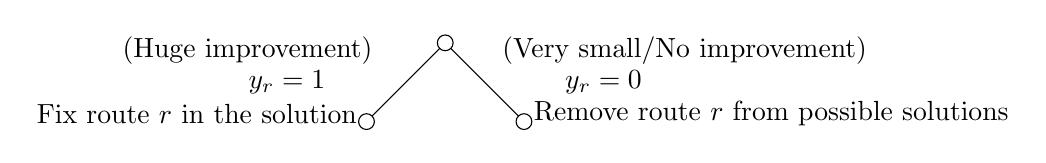
\begin{tikzpicture}[scale=0.2]
                \draw (0, 5) circle [radius=0.5];
                \draw (-5, 0) circle [radius=0.5];
                \draw (5, 0) circle [radius=0.5];
                \draw (0.353, 4.647) -- (4.647, 0.353);
                \draw (-0.353, 4.647) -- (-4.647, 0.353);
                \node [left] at (-7, 2.5) {$y_r = 1$};
                \node [left] at (-5, 0.5) { Fix route $r$ in the solution};
                \node [left] at (-4, 4.5) { (Huge improvement) };
                \node [right] at (7, 2.5) {$y_r = 0$};
                \node [right] at (5, 0.5) { Remove route $r$ from possible solutions};
                \node [right] at (3, 4.5) { (Very small/No improvement) };
            \end{tikzpicture}
        \end{figure}

        The right sub-tree will continue to be searched very inefficiently, due to the unbalance of the tree. The good news is, there are possible improvements to this issue by applying different branching strategies. One of them is the Ryan-Foster Branching Rule, which is designed for the Set Covering Problem. For any fractional solution, there are at least two elements $(i,j)$ so that $i$ and $j$ are both partially covered by the same set $S$, but there is another set $T$ that only covers $i$
        \begin{figure}[h!]
            \centering
            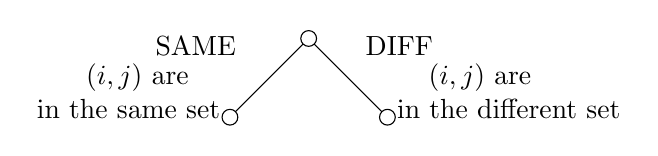
\begin{tikzpicture}[scale=0.2]
                \draw (0, 5) circle [radius=0.5];
                \draw (-5, 0) circle [radius=0.5];
                \draw (5, 0) circle [radius=0.5];
                \draw (0.353, 4.647) -- (4.647, 0.353);
                \draw (-0.353, 4.647) -- (-4.647, 0.353);
                \node [left] at (-7, 2.5) {$(i,j)$ are};
                \node [left] at (-5, 0.5) { in the same set};
                \node [left] at (-4, 4.5) {SAME};
                \node [right] at (7, 2.5) {$(i,j)$ are};
                \node [right] at (5, 0.5) { in the different set};
                \node [right] at (3, 4.5) {DIFF};
            \end{tikzpicture}
        \end{figure}

        For the search go through the SAME branch, the following constraint will be added into the follow-up subproblems.

        \begin{equation*}
            \sum_{l: (i, l) \in E} w_{il} = \sum_{l: (j, l \in E)} w_{jl}
        \end{equation*}

        For the DIFF branch, the corresponded constraints will be

        \begin{equation*}
            \sum_{l: (i, l) \in E} w_{il} + \sum_{l: (j, l \in E)} w_{jl} \le 1
        \end{equation*}

        Second, there is a terrible symmetric issue/degeneracy issue in the subproblem - the subproblem will produce duplicate routes. One of the another solutions is for every route r in $y_r = 0$ branches, add the following constraints

        \begin{equation*}
            \sum_{(i, j) \in E, w_{ij}^r = 0, \forall r \in R^\prime} w_{ij} + \sum_{(i, j) \in E, w_{ij}^r = 1, \forall r \in R'} (1 - w_{ij}) \ge 1
        \end{equation*}

        The idea is to use the edges that have not yet been used more, and use the edges that have appeared in other edges less. (But it will still be bad...)
    
    % \section{Some Accelerating Ideas In General}
    %     \subsection{For the Master Problem}

    %     \subsection{For the Subproblems/Pricing Problems}

    %     \subsection{}

    % \bibliography{literature}
\end{document}